% Created by tikzDevice version 0.12 on 2019-02-27 11:50:34
% !TEX encoding = UTF-8 Unicode
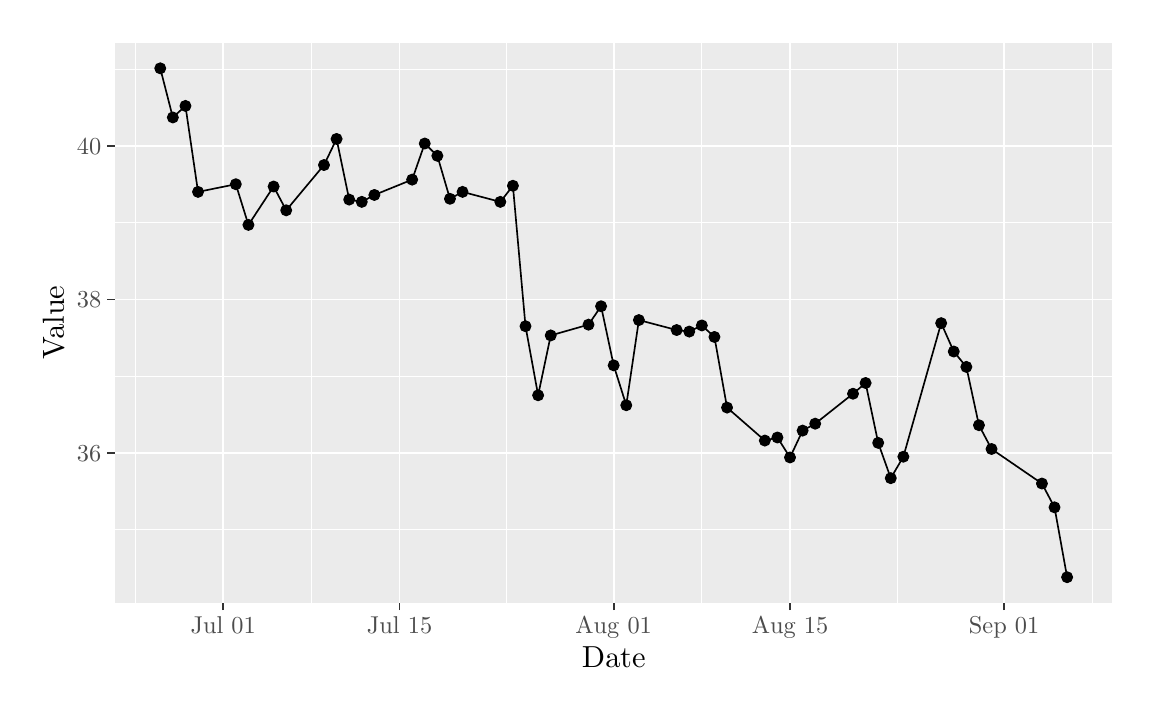
\begin{tikzpicture}[x=1pt,y=1pt]
\definecolor{fillColor}{RGB}{255,255,255}
\path[use as bounding box,fill=fillColor,fill opacity=0.00] (0,0) rectangle (397.48,238.49);
\begin{scope}
\path[clip] (  0.00,  0.00) rectangle (397.48,238.49);
\definecolor{drawColor}{RGB}{255,255,255}
\definecolor{fillColor}{RGB}{255,255,255}

\path[draw=drawColor,line width= 0.6pt,line join=round,line cap=round,fill=fillColor] (  0.00,  0.00) rectangle (397.48,238.49);
\end{scope}
\begin{scope}
\path[clip] ( 31.52, 30.73) rectangle (391.98,232.99);
\definecolor{fillColor}{gray}{0.92}

\path[fill=fillColor] ( 31.52, 30.73) rectangle (391.98,232.99);
\definecolor{drawColor}{RGB}{255,255,255}

\path[draw=drawColor,line width= 0.3pt,line join=round] ( 31.52, 57.12) --
	(391.98, 57.12);

\path[draw=drawColor,line width= 0.3pt,line join=round] ( 31.52,112.58) --
	(391.98,112.58);

\path[draw=drawColor,line width= 0.3pt,line join=round] ( 31.52,168.05) --
	(391.98,168.05);

\path[draw=drawColor,line width= 0.3pt,line join=round] ( 31.52,223.52) --
	(391.98,223.52);

\path[draw=drawColor,line width= 0.3pt,line join=round] ( 38.80, 30.73) --
	( 38.80,232.99);

\path[draw=drawColor,line width= 0.3pt,line join=round] (102.52, 30.73) --
	(102.52,232.99);

\path[draw=drawColor,line width= 0.3pt,line join=round] (173.07, 30.73) --
	(173.07,232.99);

\path[draw=drawColor,line width= 0.3pt,line join=round] (243.61, 30.73) --
	(243.61,232.99);

\path[draw=drawColor,line width= 0.3pt,line join=round] (314.16, 30.73) --
	(314.16,232.99);

\path[draw=drawColor,line width= 0.3pt,line join=round] (384.70, 30.73) --
	(384.70,232.99);

\path[draw=drawColor,line width= 0.6pt,line join=round] ( 31.52, 84.85) --
	(391.98, 84.85);

\path[draw=drawColor,line width= 0.6pt,line join=round] ( 31.52,140.32) --
	(391.98,140.32);

\path[draw=drawColor,line width= 0.6pt,line join=round] ( 31.52,195.79) --
	(391.98,195.79);

\path[draw=drawColor,line width= 0.6pt,line join=round] ( 70.66, 30.73) --
	( 70.66,232.99);

\path[draw=drawColor,line width= 0.6pt,line join=round] (134.38, 30.73) --
	(134.38,232.99);

\path[draw=drawColor,line width= 0.6pt,line join=round] (211.75, 30.73) --
	(211.75,232.99);

\path[draw=drawColor,line width= 0.6pt,line join=round] (275.47, 30.73) --
	(275.47,232.99);

\path[draw=drawColor,line width= 0.6pt,line join=round] (352.84, 30.73) --
	(352.84,232.99);
\definecolor{drawColor}{RGB}{0,0,0}

\path[draw=drawColor,line width= 0.6pt,line join=round] ( 47.91,223.80) --
	( 52.46,206.05) --
	( 57.01,210.21) --
	( 61.56,179.15) --
	( 75.21,181.92) --
	( 79.77,167.22) --
	( 88.87,181.09) --
	( 93.42,172.49) --
	(107.07,188.85) --
	(111.62,198.28) --
	(116.18,176.37) --
	(120.73,175.54) --
	(125.28,178.04) --
	(138.93,183.58) --
	(143.48,196.62) --
	(148.04,192.18) --
	(152.59,176.65) --
	(157.14,179.15) --
	(170.79,175.54) --
	(175.34,181.36) --
	(179.89,130.61) --
	(184.45,105.65) --
	(189.00,127.28) --
	(202.65,131.17) --
	(207.20,137.82) --
	(211.75,116.47) --
	(216.30,102.05) --
	(220.86,132.83) --
	(234.51,129.23) --
	(239.06,128.67) --
	(243.61,130.89) --
	(248.16,126.73) --
	(252.72,101.21) --
	(266.37, 89.29) --
	(270.92, 90.40) --
	(275.47, 83.19) --
	(280.02, 92.89) --
	(284.57, 95.39) --
	(298.23,106.21) --
	(302.78,110.09) --
	(307.33, 88.46) --
	(311.88, 75.70) --
	(316.43, 83.46) --
	(330.09,131.72) --
	(334.64,121.46) --
	(339.19,115.91) --
	(343.74, 94.84) --
	(348.29, 86.24) --
	(366.50, 73.76) --
	(371.05, 65.16) --
	(375.60, 39.92);
\definecolor{fillColor}{RGB}{0,0,0}

\path[draw=drawColor,line width= 0.4pt,line join=round,line cap=round,fill=fillColor] ( 47.91,223.80) circle (  1.96);

\path[draw=drawColor,line width= 0.4pt,line join=round,line cap=round,fill=fillColor] ( 52.46,206.05) circle (  1.96);

\path[draw=drawColor,line width= 0.4pt,line join=round,line cap=round,fill=fillColor] ( 57.01,210.21) circle (  1.96);

\path[draw=drawColor,line width= 0.4pt,line join=round,line cap=round,fill=fillColor] ( 61.56,179.15) circle (  1.96);

\path[draw=drawColor,line width= 0.4pt,line join=round,line cap=round,fill=fillColor] ( 75.21,181.92) circle (  1.96);

\path[draw=drawColor,line width= 0.4pt,line join=round,line cap=round,fill=fillColor] ( 79.77,167.22) circle (  1.96);

\path[draw=drawColor,line width= 0.4pt,line join=round,line cap=round,fill=fillColor] ( 88.87,181.09) circle (  1.96);

\path[draw=drawColor,line width= 0.4pt,line join=round,line cap=round,fill=fillColor] ( 93.42,172.49) circle (  1.96);

\path[draw=drawColor,line width= 0.4pt,line join=round,line cap=round,fill=fillColor] (107.07,188.85) circle (  1.96);

\path[draw=drawColor,line width= 0.4pt,line join=round,line cap=round,fill=fillColor] (111.62,198.28) circle (  1.96);

\path[draw=drawColor,line width= 0.4pt,line join=round,line cap=round,fill=fillColor] (116.18,176.37) circle (  1.96);

\path[draw=drawColor,line width= 0.4pt,line join=round,line cap=round,fill=fillColor] (120.73,175.54) circle (  1.96);

\path[draw=drawColor,line width= 0.4pt,line join=round,line cap=round,fill=fillColor] (125.28,178.04) circle (  1.96);

\path[draw=drawColor,line width= 0.4pt,line join=round,line cap=round,fill=fillColor] (138.93,183.58) circle (  1.96);

\path[draw=drawColor,line width= 0.4pt,line join=round,line cap=round,fill=fillColor] (143.48,196.62) circle (  1.96);

\path[draw=drawColor,line width= 0.4pt,line join=round,line cap=round,fill=fillColor] (148.04,192.18) circle (  1.96);

\path[draw=drawColor,line width= 0.4pt,line join=round,line cap=round,fill=fillColor] (152.59,176.65) circle (  1.96);

\path[draw=drawColor,line width= 0.4pt,line join=round,line cap=round,fill=fillColor] (157.14,179.15) circle (  1.96);

\path[draw=drawColor,line width= 0.4pt,line join=round,line cap=round,fill=fillColor] (170.79,175.54) circle (  1.96);

\path[draw=drawColor,line width= 0.4pt,line join=round,line cap=round,fill=fillColor] (175.34,181.36) circle (  1.96);

\path[draw=drawColor,line width= 0.4pt,line join=round,line cap=round,fill=fillColor] (179.89,130.61) circle (  1.96);

\path[draw=drawColor,line width= 0.4pt,line join=round,line cap=round,fill=fillColor] (184.45,105.65) circle (  1.96);

\path[draw=drawColor,line width= 0.4pt,line join=round,line cap=round,fill=fillColor] (189.00,127.28) circle (  1.96);

\path[draw=drawColor,line width= 0.4pt,line join=round,line cap=round,fill=fillColor] (202.65,131.17) circle (  1.96);

\path[draw=drawColor,line width= 0.4pt,line join=round,line cap=round,fill=fillColor] (207.20,137.82) circle (  1.96);

\path[draw=drawColor,line width= 0.4pt,line join=round,line cap=round,fill=fillColor] (211.75,116.47) circle (  1.96);

\path[draw=drawColor,line width= 0.4pt,line join=round,line cap=round,fill=fillColor] (216.30,102.05) circle (  1.96);

\path[draw=drawColor,line width= 0.4pt,line join=round,line cap=round,fill=fillColor] (220.86,132.83) circle (  1.96);

\path[draw=drawColor,line width= 0.4pt,line join=round,line cap=round,fill=fillColor] (234.51,129.23) circle (  1.96);

\path[draw=drawColor,line width= 0.4pt,line join=round,line cap=round,fill=fillColor] (239.06,128.67) circle (  1.96);

\path[draw=drawColor,line width= 0.4pt,line join=round,line cap=round,fill=fillColor] (243.61,130.89) circle (  1.96);

\path[draw=drawColor,line width= 0.4pt,line join=round,line cap=round,fill=fillColor] (248.16,126.73) circle (  1.96);

\path[draw=drawColor,line width= 0.4pt,line join=round,line cap=round,fill=fillColor] (252.72,101.21) circle (  1.96);

\path[draw=drawColor,line width= 0.4pt,line join=round,line cap=round,fill=fillColor] (266.37, 89.29) circle (  1.96);

\path[draw=drawColor,line width= 0.4pt,line join=round,line cap=round,fill=fillColor] (270.92, 90.40) circle (  1.96);

\path[draw=drawColor,line width= 0.4pt,line join=round,line cap=round,fill=fillColor] (275.47, 83.19) circle (  1.96);

\path[draw=drawColor,line width= 0.4pt,line join=round,line cap=round,fill=fillColor] (280.02, 92.89) circle (  1.96);

\path[draw=drawColor,line width= 0.4pt,line join=round,line cap=round,fill=fillColor] (284.57, 95.39) circle (  1.96);

\path[draw=drawColor,line width= 0.4pt,line join=round,line cap=round,fill=fillColor] (298.23,106.21) circle (  1.96);

\path[draw=drawColor,line width= 0.4pt,line join=round,line cap=round,fill=fillColor] (302.78,110.09) circle (  1.96);

\path[draw=drawColor,line width= 0.4pt,line join=round,line cap=round,fill=fillColor] (307.33, 88.46) circle (  1.96);

\path[draw=drawColor,line width= 0.4pt,line join=round,line cap=round,fill=fillColor] (311.88, 75.70) circle (  1.96);

\path[draw=drawColor,line width= 0.4pt,line join=round,line cap=round,fill=fillColor] (316.43, 83.46) circle (  1.96);

\path[draw=drawColor,line width= 0.4pt,line join=round,line cap=round,fill=fillColor] (330.09,131.72) circle (  1.96);

\path[draw=drawColor,line width= 0.4pt,line join=round,line cap=round,fill=fillColor] (334.64,121.46) circle (  1.96);

\path[draw=drawColor,line width= 0.4pt,line join=round,line cap=round,fill=fillColor] (339.19,115.91) circle (  1.96);

\path[draw=drawColor,line width= 0.4pt,line join=round,line cap=round,fill=fillColor] (343.74, 94.84) circle (  1.96);

\path[draw=drawColor,line width= 0.4pt,line join=round,line cap=round,fill=fillColor] (348.29, 86.24) circle (  1.96);

\path[draw=drawColor,line width= 0.4pt,line join=round,line cap=round,fill=fillColor] (366.50, 73.76) circle (  1.96);

\path[draw=drawColor,line width= 0.4pt,line join=round,line cap=round,fill=fillColor] (371.05, 65.16) circle (  1.96);

\path[draw=drawColor,line width= 0.4pt,line join=round,line cap=round,fill=fillColor] (375.60, 39.92) circle (  1.96);
\end{scope}
\begin{scope}
\path[clip] (  0.00,  0.00) rectangle (397.48,238.49);
\definecolor{drawColor}{gray}{0.30}

\node[text=drawColor,anchor=base east,inner sep=0pt, outer sep=0pt, scale=  0.88] at ( 26.57, 81.82) {36};

\node[text=drawColor,anchor=base east,inner sep=0pt, outer sep=0pt, scale=  0.88] at ( 26.57,137.29) {38};

\node[text=drawColor,anchor=base east,inner sep=0pt, outer sep=0pt, scale=  0.88] at ( 26.57,192.76) {40};
\end{scope}
\begin{scope}
\path[clip] (  0.00,  0.00) rectangle (397.48,238.49);
\definecolor{drawColor}{gray}{0.20}

\path[draw=drawColor,line width= 0.6pt,line join=round] ( 28.77, 84.85) --
	( 31.52, 84.85);

\path[draw=drawColor,line width= 0.6pt,line join=round] ( 28.77,140.32) --
	( 31.52,140.32);

\path[draw=drawColor,line width= 0.6pt,line join=round] ( 28.77,195.79) --
	( 31.52,195.79);
\end{scope}
\begin{scope}
\path[clip] (  0.00,  0.00) rectangle (397.48,238.49);
\definecolor{drawColor}{gray}{0.20}

\path[draw=drawColor,line width= 0.6pt,line join=round] ( 70.66, 27.98) --
	( 70.66, 30.73);

\path[draw=drawColor,line width= 0.6pt,line join=round] (134.38, 27.98) --
	(134.38, 30.73);

\path[draw=drawColor,line width= 0.6pt,line join=round] (211.75, 27.98) --
	(211.75, 30.73);

\path[draw=drawColor,line width= 0.6pt,line join=round] (275.47, 27.98) --
	(275.47, 30.73);

\path[draw=drawColor,line width= 0.6pt,line join=round] (352.84, 27.98) --
	(352.84, 30.73);
\end{scope}
\begin{scope}
\path[clip] (  0.00,  0.00) rectangle (397.48,238.49);
\definecolor{drawColor}{gray}{0.30}

\node[text=drawColor,anchor=base,inner sep=0pt, outer sep=0pt, scale=  0.88] at ( 70.66, 19.72) {Jul 01};

\node[text=drawColor,anchor=base,inner sep=0pt, outer sep=0pt, scale=  0.88] at (134.38, 19.72) {Jul 15};

\node[text=drawColor,anchor=base,inner sep=0pt, outer sep=0pt, scale=  0.88] at (211.75, 19.72) {Aug 01};

\node[text=drawColor,anchor=base,inner sep=0pt, outer sep=0pt, scale=  0.88] at (275.47, 19.72) {Aug 15};

\node[text=drawColor,anchor=base,inner sep=0pt, outer sep=0pt, scale=  0.88] at (352.84, 19.72) {Sep 01};
\end{scope}
\begin{scope}
\path[clip] (  0.00,  0.00) rectangle (397.48,238.49);
\definecolor{drawColor}{RGB}{0,0,0}

\node[text=drawColor,anchor=base,inner sep=0pt, outer sep=0pt, scale=  1.10] at (211.75,  7.44) {Date};
\end{scope}
\begin{scope}
\path[clip] (  0.00,  0.00) rectangle (397.48,238.49);
\definecolor{drawColor}{RGB}{0,0,0}

\node[text=drawColor,rotate= 90.00,anchor=base,inner sep=0pt, outer sep=0pt, scale=  1.10] at ( 13.08,131.86) {Value};
\end{scope}
\end{tikzpicture}
